In this section we consider the dynamics of two interacting hypercolumns, each one made of two minicolumns. The model considered is the rBCPNN in \cref{rBCPNN}. In particular we investigate how the symmetric, mutual interaction between the two modular units, together with the self excitation, shape the qualitative behaviour of the system. We will assume the coupling  weights to be static, result of a previous learning experience. This first analysis heavily exploits the properties of Monotone Control Systems as introduced in \cite{angeli2003monotone} and in particular the reduction theorem proposed in \cite{enciso2005monotone}. We will show how the interaction matrices learned with the hebbian learning rule make the system monotone according to the right choice of cones and orthants (refer to the Preliminaries section). Furthermore the monotonicity approach will be compared with the Lyapunov Stability approach.

\subsection{Monotonicity Analysis}
Denote $s_{11}, s_{12}, s_{21}, s_{22}$ the activities of the minicolumns grouped in the two hypercolumns $s_1 = [s_{11}, s_{12}]^T$ and $s_2 = [s_{21}, s_{22}]^T$;  $o_1 = [o_{11}, o_{12}]^T$ and $o_2 = [o_{21}, o_{22}]^T$ the corresponding outputs computed withe softmax distribution; $\beta_1 = [\beta_{11}, \beta_{12}]$, $\beta_2 = [\beta_{21}, \beta_{22}]$ the self excitation biases; $W$ the interaction matrix between the two units. The interactions are symmetric in the sense that the coupling factor between unit $i$ and unit $j$ is equal to the coupling factor between unit $j$ and unit $i$. The system dynamics follows in the compact form:

\begin{equation}
\begin{aligned}
\tau_m \dot{s_1} &= \beta_{1} + Wo_{2}-s_{1} \\
\tau_m \dot{s_2} &= \beta_{2} + W^{T}o_{1}-s_{2} \\
W & =
\begin{bmatrix}
 w_{1121} & w_{1122} \\
 w_{1221} & w_{1222} \\
\end{bmatrix} = 
\begin{bmatrix}
 w_{1} & w_{2} \\
 w_{3} & w_{4} \\
\end{bmatrix} 
\end{aligned}
\label{eq:cl_loop}
\end{equation}
By defining $y = o_1$ we can see our system in \eqref{eq:cl_loop} as the closed loop system which arises under unitary output feedback for the following system with inputs and outputs:

\begin{equation}
\begin{aligned}
\tau_m \dot{s_1} &= \beta_{1} + Wo_{2}-s_{1} \\
\tau_m \dot{s_2} &= \beta_{2} + W^{T}u-s_{2} \\
y & = h(s_1, s_2) = o_1
\end{aligned}
\label{eq:op_loop}
\end{equation}

This simple trick will allow us, by using the main result in \cite{enciso2005monotone} to determine the number of asymptotically stable points (attractors) of system in \eqref{eq:cl_loop} by studying a reduced order continuous-time system. The system in \eqref{eq:op_loop} is a monotone system according to definition to be defined. In fact ...

Furthermore, we have to show that   the closed loop system in \eqref{eq:cl_loop} is a monotone system with respect to the right choice of orthants (refer to the section on monotone systems). In order to do so we compute the jacobian matrix for the dynamics in \eqref{eq:cl_loop}.
\begin{equation}
\begin{aligned}
\frac{\partial s_{11}}{\partial s_{21}} &= e^{s_{22}} \frac{e^{s_{21}}(w_{1121} - w_{1122}) + w_{1121}e^{s_{22}}    }{e^{s_{21}}(e^{s_{21}}+ e^{s_{22}})} 
\end{aligned}
\label{eq:jac_s1121}
\end{equation}


\begin{equation}
\begin{aligned}
\frac{\partial s_{11}}{\partial s_{22}} &= e^{s_{21}} \frac{e^{s_{22}}(w_{1122} - w_{1121}) + w_{1122}e^{s_{21}}    }{e^{s_{22}}(e^{s_{22}}+ e^{s_{21}})} 
\end{aligned}
\label{eq:jac_s1122}
\end{equation}


\begin{equation}
\begin{aligned}
\frac{\partial s_{12}}{\partial s_{21}} &= e^{s_{22}} \frac{e^{s_{21}}(w_{1221} - w_{1222}) + w_{1221}e^{s_{22}}    }{e^{s_{21}}(e^{s_{21}}+ e^{s_{22}})} 
\end{aligned}
\label{eq:jac_s1221}
\end{equation}


\begin{equation}
\begin{aligned}
\frac{\partial s_{12}}{\partial s_{22}} &= e^{s_{21}} \frac{e^{s_{22}}(w_{1222} - w_{1221}) + w_{1222}e^{s_{21}}    }{e^{s_{22}}(e^{s_{22}}+ e^{s_{21}})} 
\end{aligned}
\label{eq:jac_s1222}
\end{equation}
Analogous results are obtained for $\frac{\partial s_{21}}{\partial s_{11}}, \frac{\partial s_{21}}{\partial s_{12}}, \frac{\partial s_{22}}{\partial s_{11}}, \frac{\partial s_{22}}{\partial s_{12}}$. 

For the following analysis we will assume that during the learning procedure a unique pattern is presented to the network. As explained in (cite section on learning procedure), the pattern is 'fixed' into the network by clamping the input units and leaving the matrix weights adapt. For this first preliminary analysis we will assume that the input current is such that the outputs $o_1 \approx [1 , 0]^T$ and $o_2 \approx [1, 0]^T$. According to the equation in \eqref{eq:wij} and assuming that $p_{11} = p_{21} \approx 1$, $p_{12} = p_{22} \approx 0$ a suitable choice for the matrix weights $W$ is the following:  

\begin{equation}
W = \begin{bmatrix}
 0 & -\alpha \\
 -\alpha & 0 \\
\end{bmatrix},\  \alpha = - log(\epsilon) >0
\label{eq:coup_eps_matrix}
\end{equation}
With this particular choice, the partial derivatives above have 'well-defined-sign'(find the right expression) everywhere in the state space and we can write:

\begin{equation}
\begin{aligned}
\frac{\partial s_{11}}{\partial s_{21}} & > 0, & 
\frac{\partial s_{11}}{\partial s_{22}} & < 0, & \frac{\partial s_{12}}{\partial s_{21}} &< 0, & \frac{\partial s_{12}}{\partial s_{22}}  &> 0
\end{aligned}
\end{equation}

\begin{equation}
\begin{aligned}
\frac{\partial s_{21}}{\partial s_{11}} & > 0, & 
\frac{\partial s_{21}}{\partial s_{22}} & < 0, & \frac{\partial s_{22}}{\partial s_{11}} &< 0, & \frac{\partial s_{22}}{\partial s_{12}}  &> 0
\end{aligned}
\end{equation}
By considering the partial order $\succeq$ induced on ${\rm I\!R}^4$ by the orthant $K = {\rm I\!R}_{\geq 0} \times {\rm I\!R}_{\leq 0} \times {\rm I\!R}_{\geq 0} \times {\rm I\!R}_{\leq 0}$ and by using (link to the right proposition) it follows that the closed loop in \eqref{eq:cl_loop} is a monotone systems. An alternative way to show that a system is monotone is to use the graphical conditions for monotonicity developed in \cite{angeli2004multigraph} recalled in the preliminaries section. In particular one need to show that the adjacency matrix describing the sign of the interactions between the states has no negative loops.

\paragraph{Reduced order system} 
Consider now the controlled system in \eqref{eq:op_loop}. By fixing the input $u = [u_1, u_2]^T$ the system converges to the equilibrium point that define  the I/S characteristic $k^X: U \mapsto X$:

\begin{equation}
    \begin{aligned}
    s_1^* &=  \beta_1 + W\sigma(s_2^*)\\
    s_2^* &=  \beta_2 + W^T\sigma(u)\\
    \end{aligned}
\end{equation}
By composing the I/S characteristic with the output function in \eqref{eq:cl_loop} we obtain:
\begin{equation}
    k(u) = \sigma(\beta_1 + W\sigma(W^Tu + \beta_2))
    \label{eq:reduced_2d}
\end{equation}
We can now study the following reduced order dynamics:
\begin{equation}
    \dot{u} = k(u) - u
    \label{eq:reduced_2d}
\end{equation}
In this case, the reduced order system is 2-dimensional, therefore a phase plane analysis will help us to understand the nature of equilibrium points. We will first analyse the effect of varying the coupling strength $\alpha$ in the matrix \eqref{eq:coup_eps_matrix}, then the effect of the biases $\beta_1,\beta_2$.

\paragraph{Effect of coupling strength $\alpha$} We will study the effect of varying the coupling strength by a phase portrait analysis. The bias parameters $ \beta_1, \beta_2$ will be initially assumed to be zero. In particular we can notice that by increasing the coupling factor $ \alpha $ from 0 (no coupling) to higher values, two stable equilibria emerges \cref{fig:two_d_system_eps_effect}. This is a particular case of \textbf{supercrictical pitchfork bifurcation} \cite{StrogatzNonlinear}: in fact, by varying the parameter $\alpha$, the system transitions from one (stable) fixed point to three fixed points: one unstable and two stable (\cref{fig:two_d_system_eps_effect}). 

Simulations of the original system on \eqref{eq:cl_loop} with different initial conditions show that, as expected, the qualitative behaviour (number of fixed points) of the 2-dimensional reduced order system is kept in the original 4-dimensional system. In \cref{fig:s_mono_one} and \cref{fig:s_mono_two} the evolution of states with several initial conditions, both for $\alpha=1.5$ (one equilibrium) and $\alpha=8$ (2 equilibria) is shown.

\iftrue
   \begin{figure*}
        %\centering
        \begin{subfigure}[b]{0.475\textwidth}
            \centering
            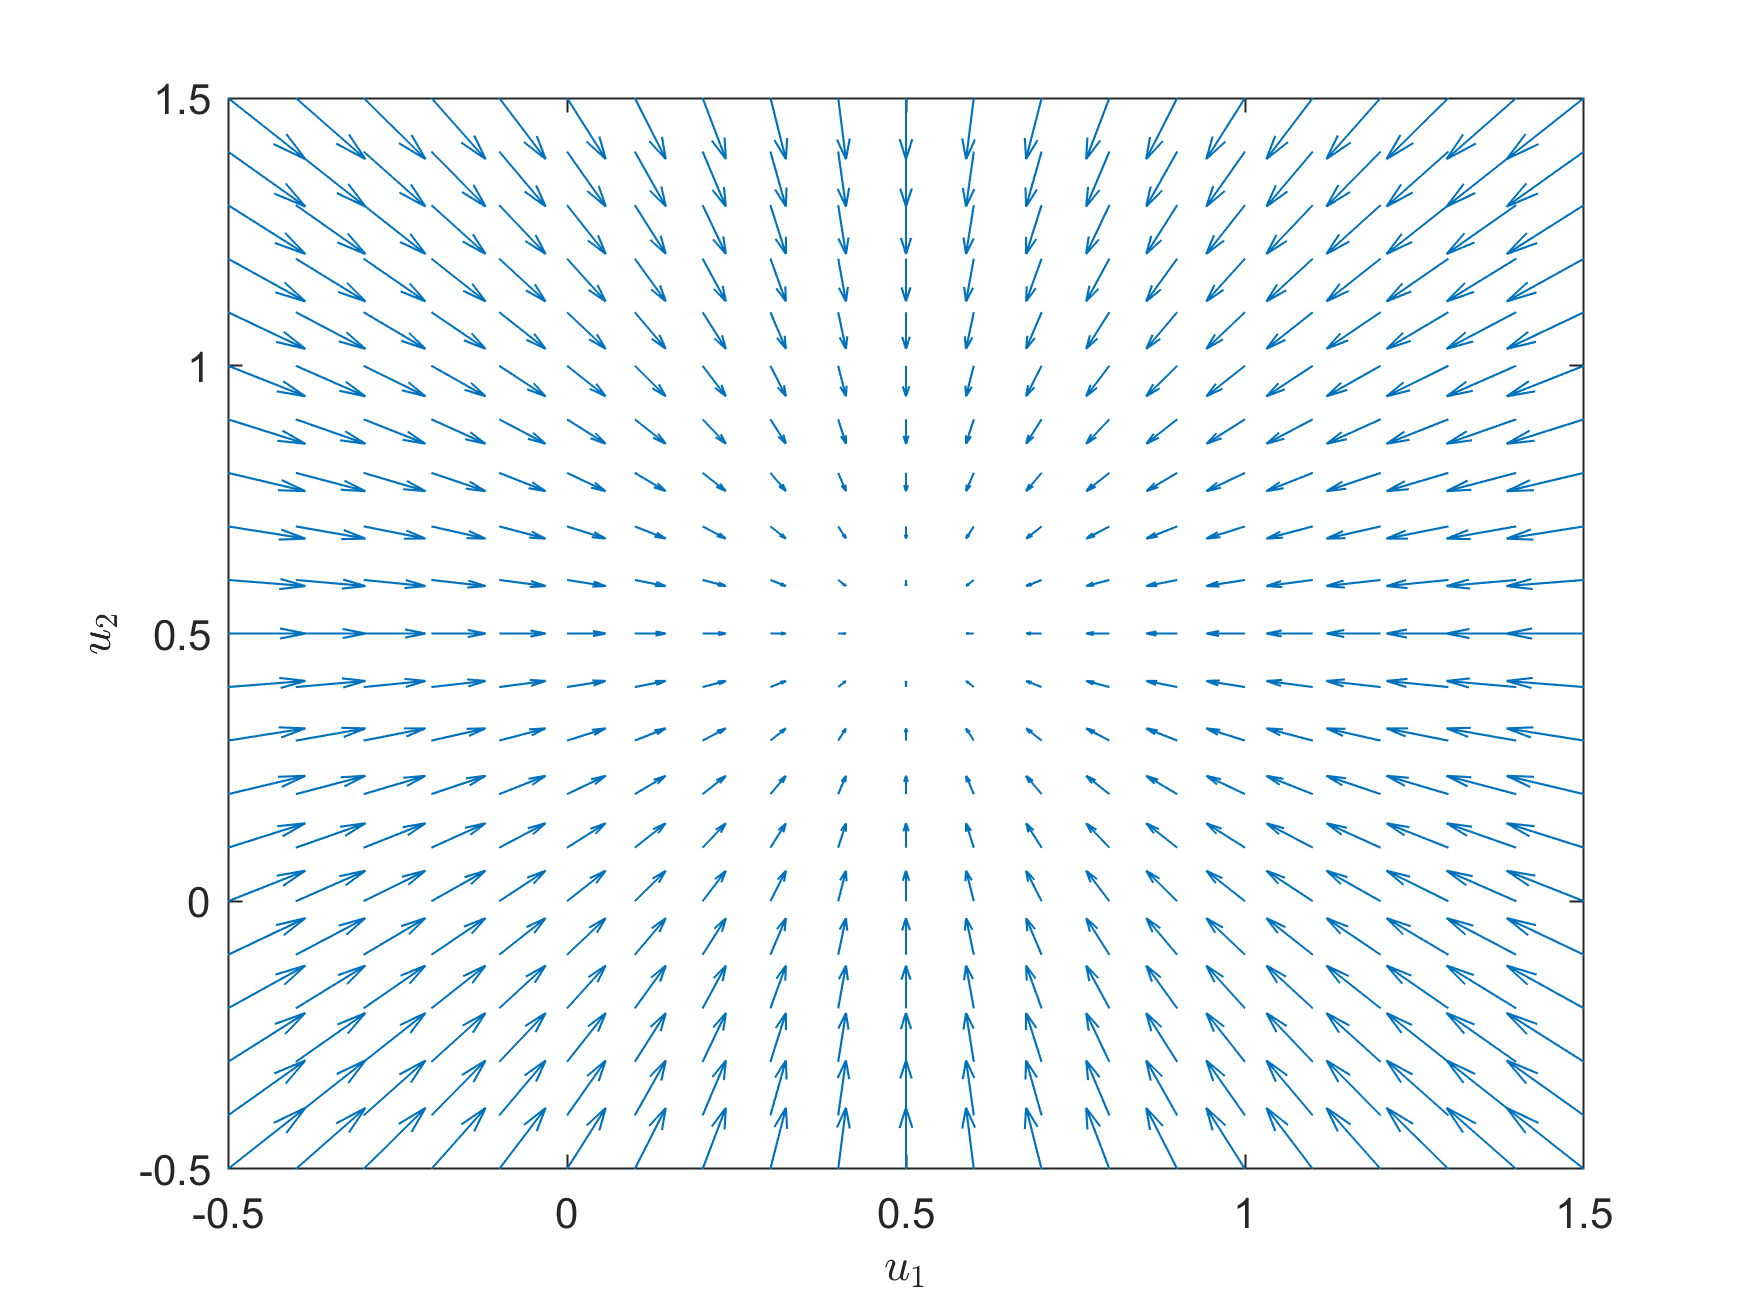
\includegraphics[width=\textwidth]{text/analysis/fig/2by2monotone/espi_0.png}
            \caption{\small $\alpha=0$}
            \label{fig:mean and std of net14}
        \end{subfigure}
        \hfill
        \begin{subfigure}[b]{0.475\textwidth}  
            \centering 
            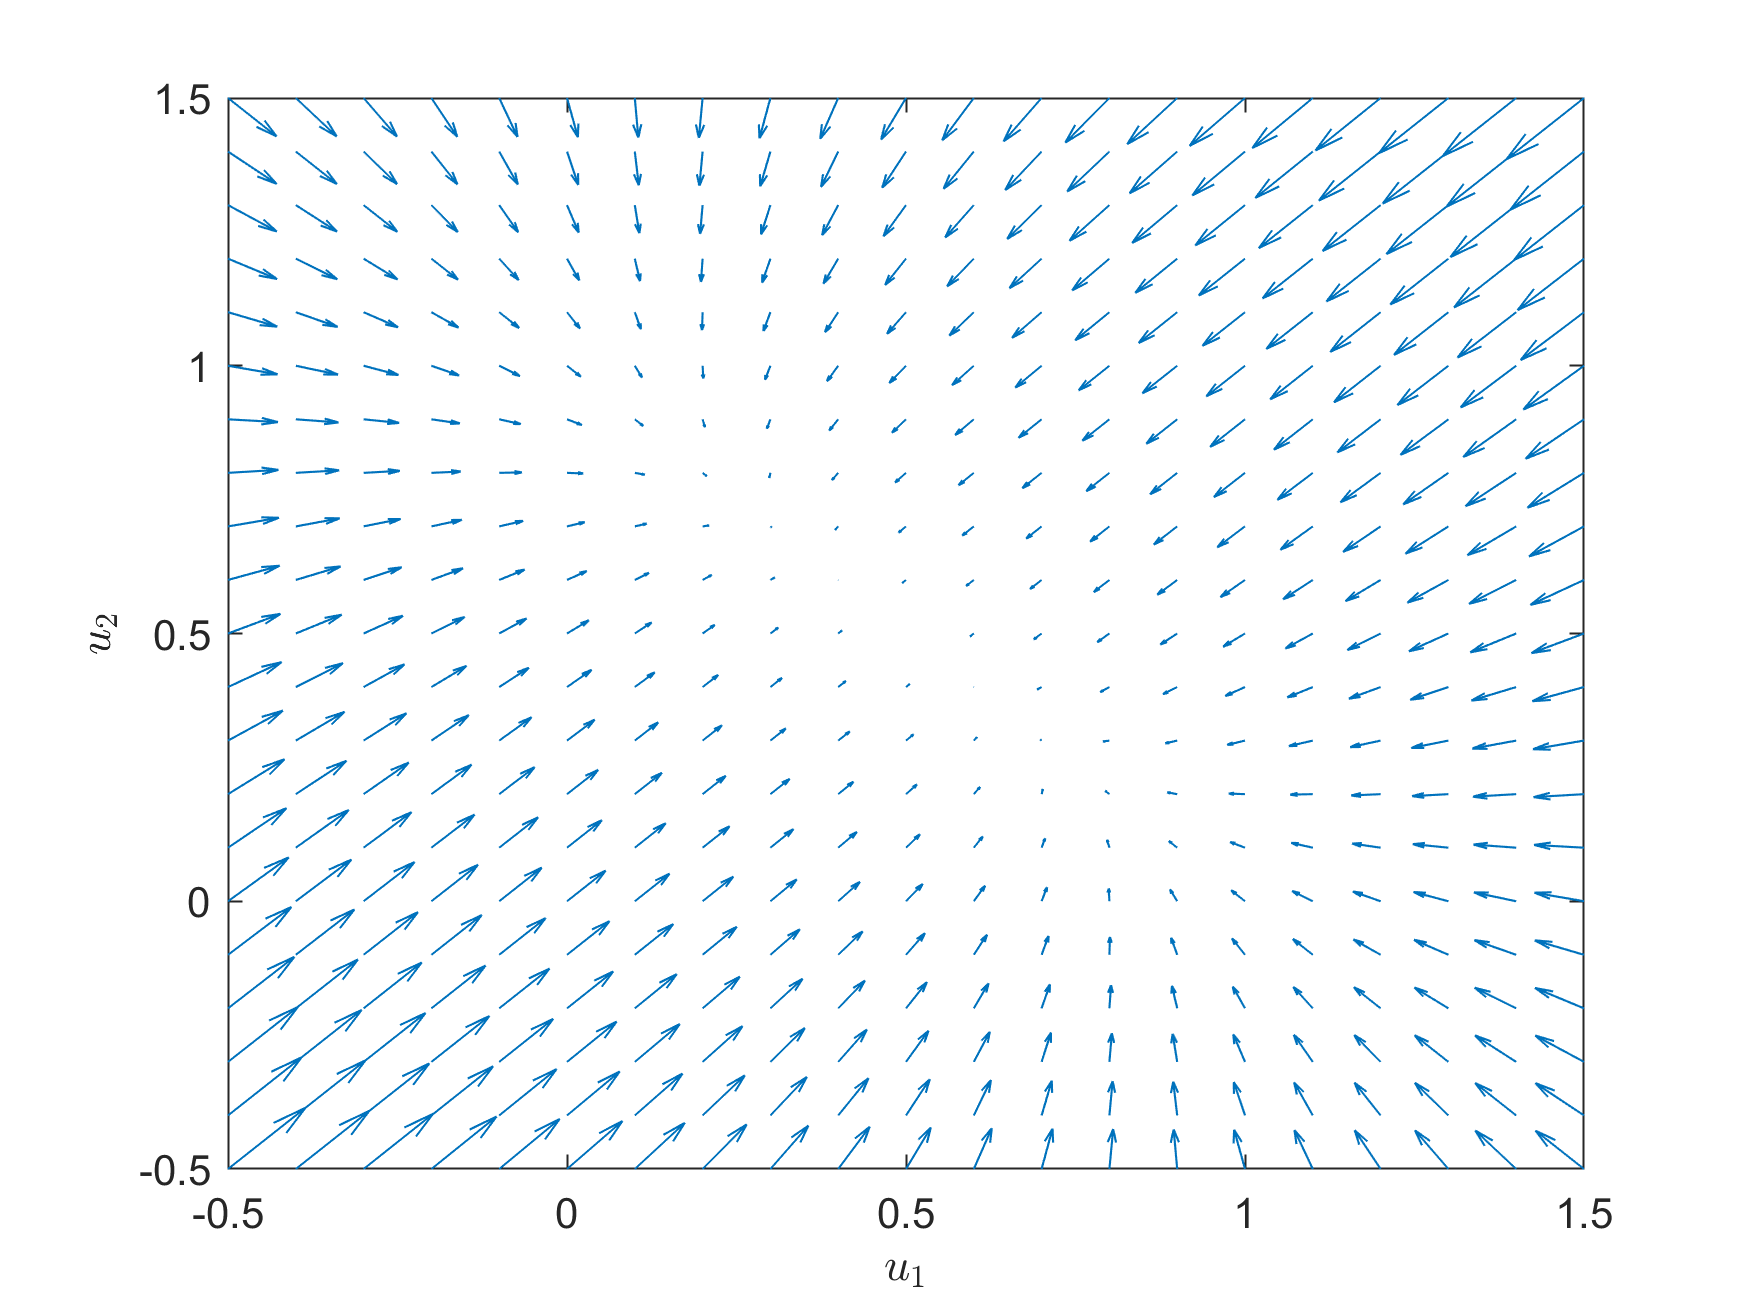
\includegraphics[width=\textwidth]{text/analysis/fig/2by2monotone/espi_2.png}
            \caption{$\alpha=2$}
            \label{fig:mean and std of net24}
        \end{subfigure}
        \vskip\baselineskip
        \begin{subfigure}[b]{0.475\textwidth}   
            \centering 
            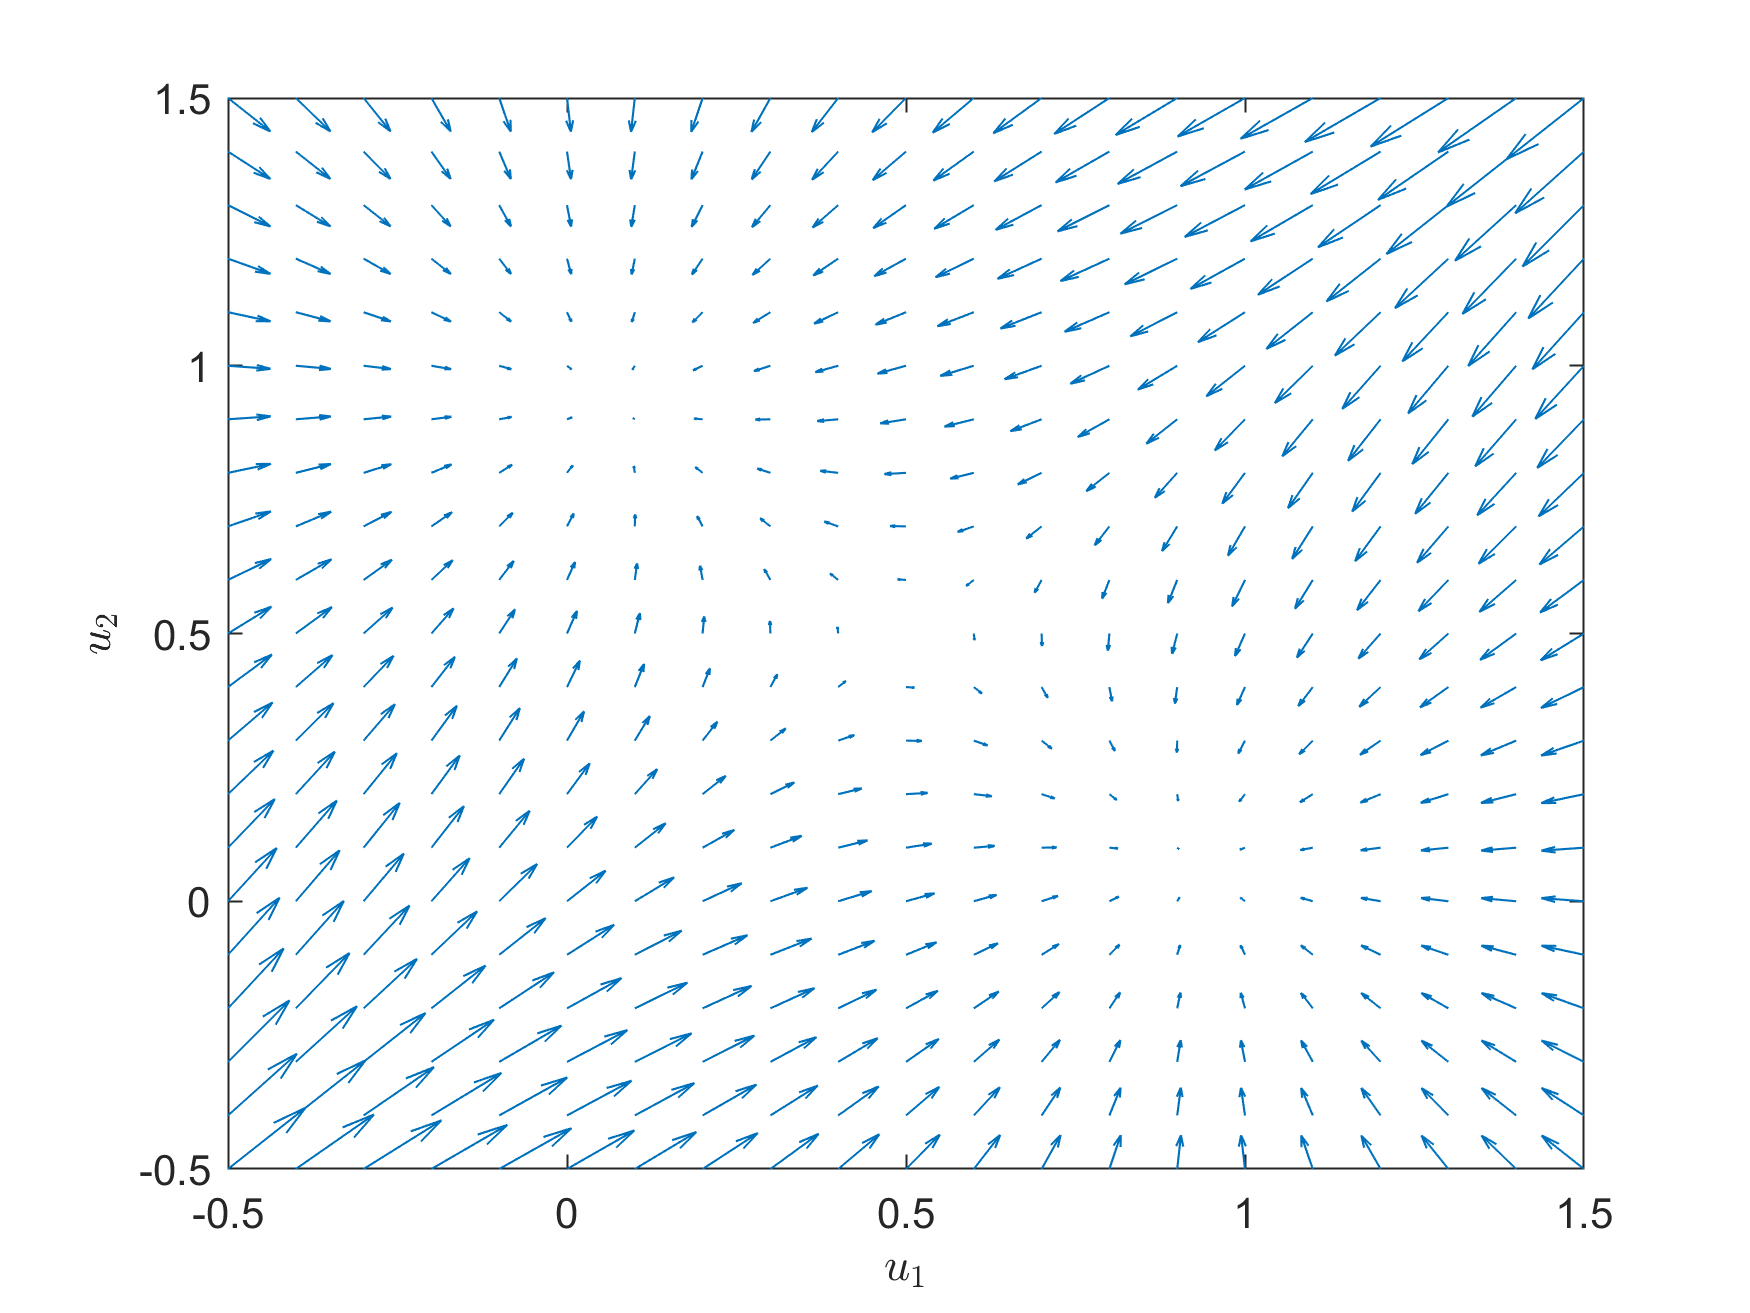
\includegraphics[width=\textwidth]{text/analysis/fig/2by2monotone/espi_3.png}
            \caption{$\alpha=3$}
            \label{fig:mean and std of net34}
        \end{subfigure}
        \quad
        \begin{subfigure}[b]{0.475\textwidth}   
            \centering 
            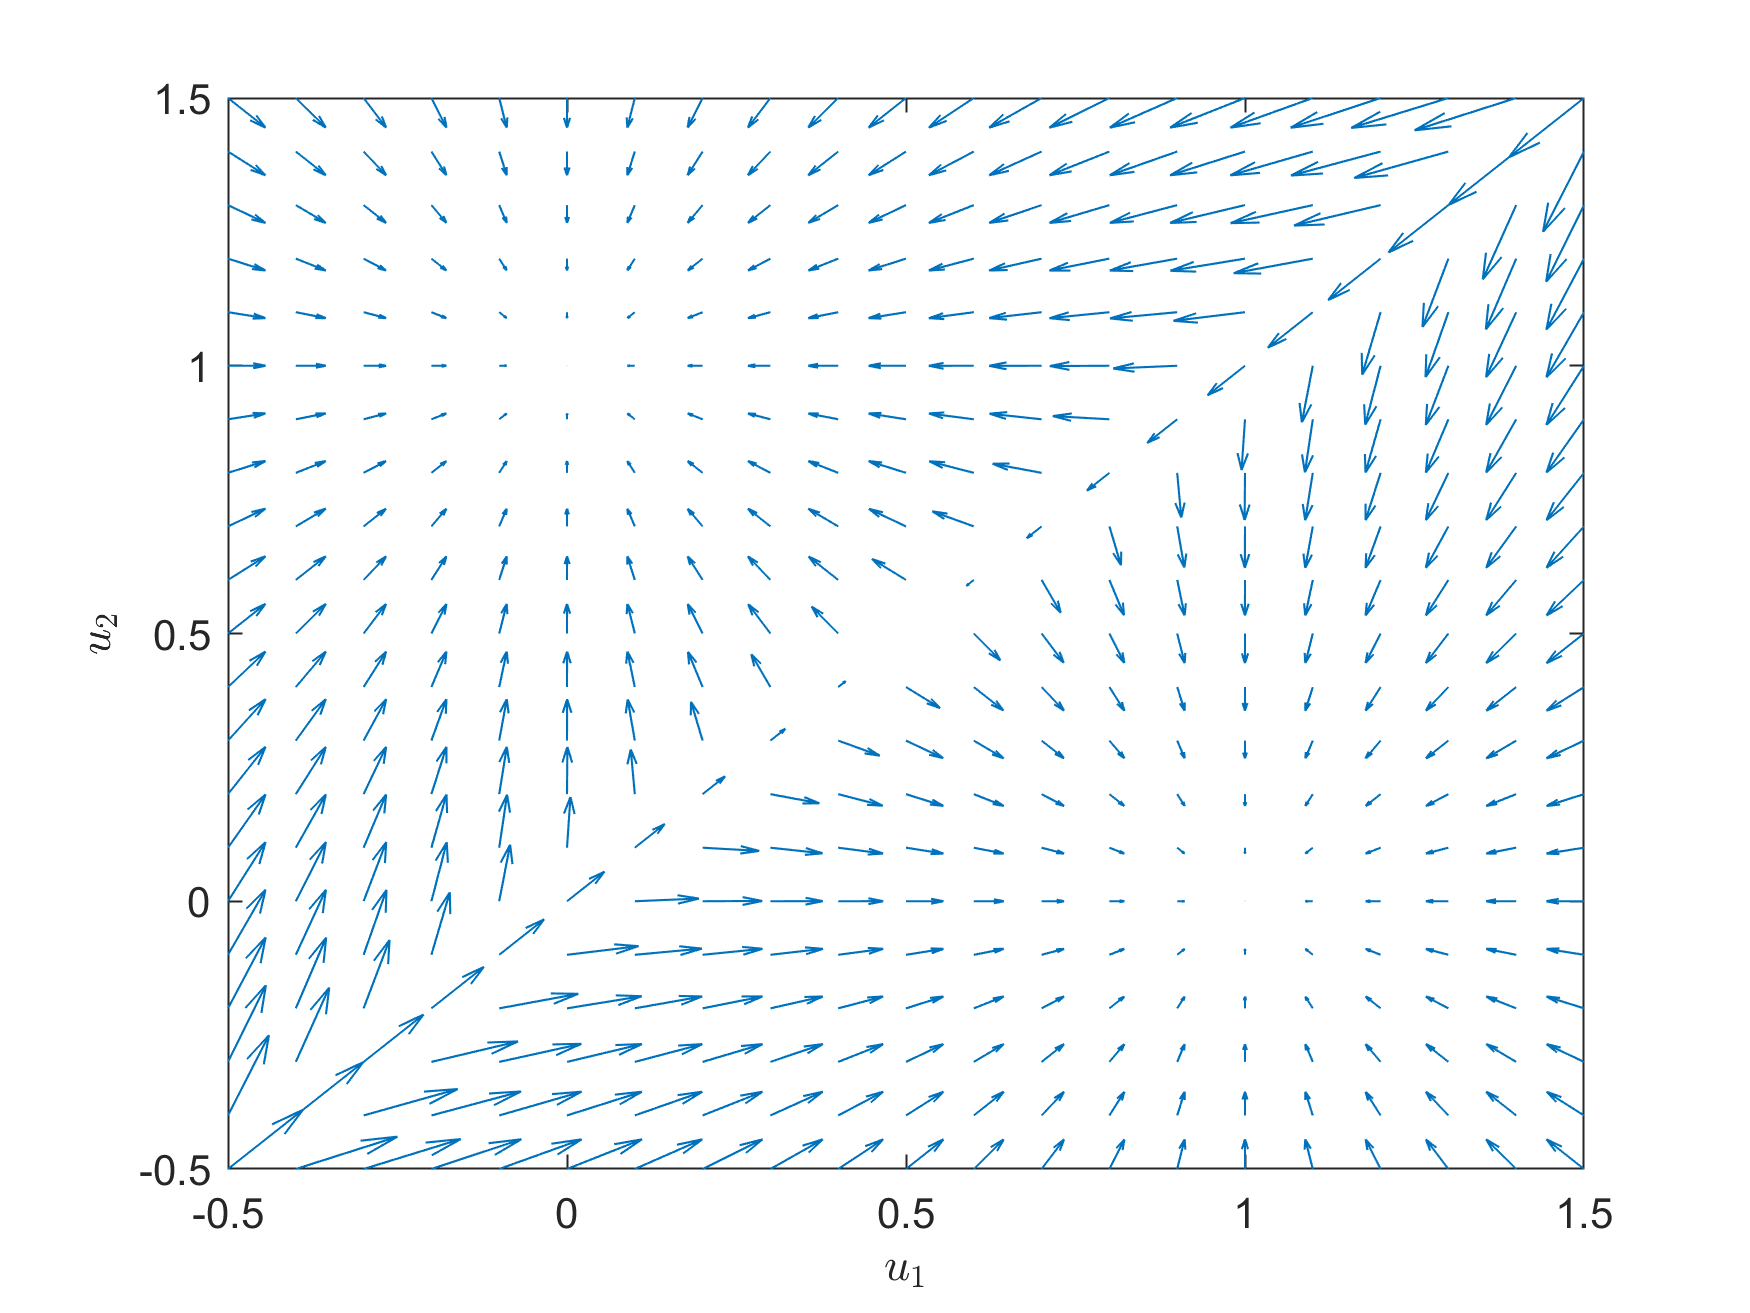
\includegraphics[width=\textwidth]{text/analysis/fig/2by2monotone/espi_8.png}
            \caption{$\alpha=8$}
            \label{fig:mean and std of net44}
        \end{subfigure}
        \caption{Phase portrait for the system in \eqref{eq:reduced_2d} with different coupling factors. $u=[u_1, u_2]^T$} 
        \label{fig:two_d_system_eps_effect}
    \end{figure*}
\fi

\begin{figure}
    \centering
    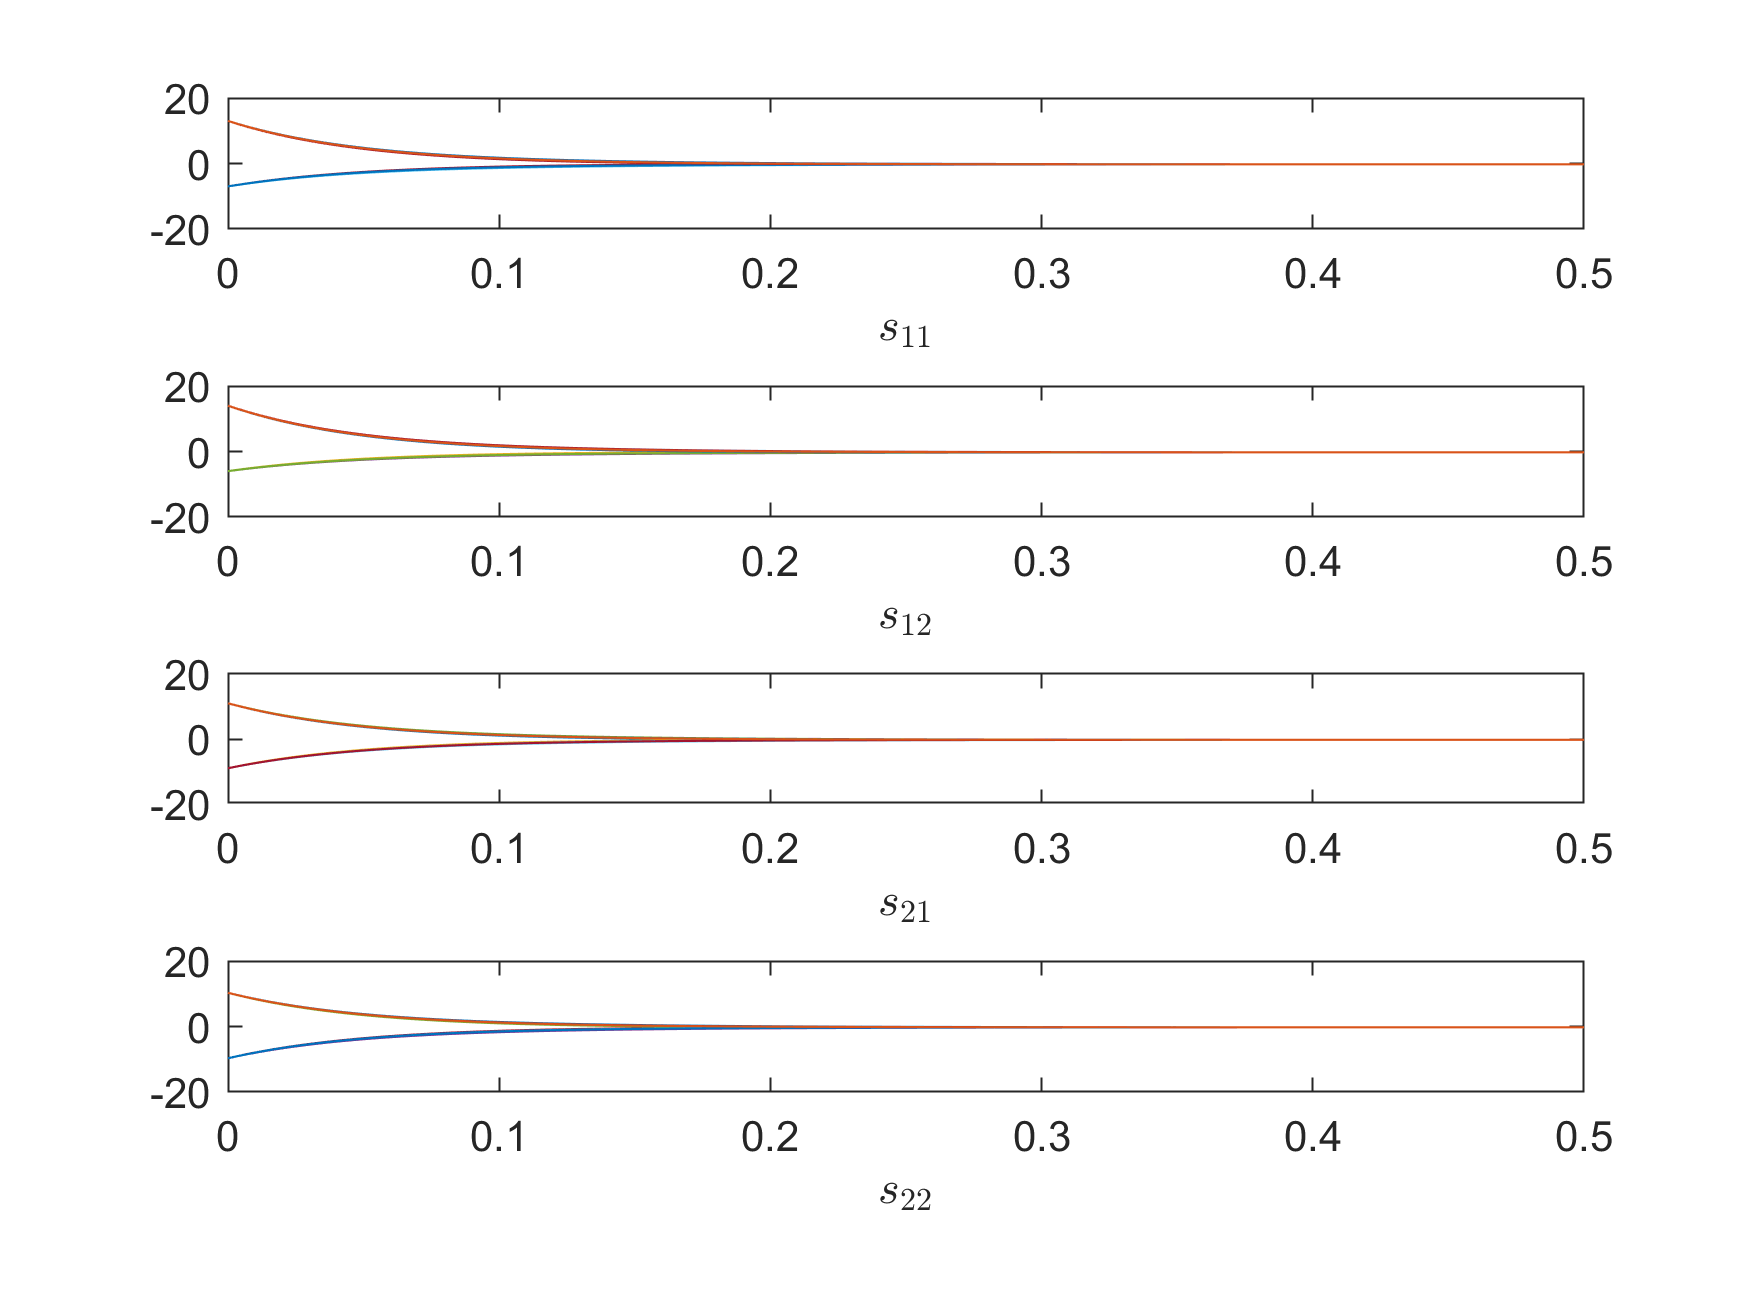
\includegraphics[width=\textwidth]{text/analysis/fig/2by2monotone/s.png}
    \caption{Original system \eqref{eq:cl_loop} simulation with several initial conditions}
    \label{fig:s_mono_one}
\end{figure}
    
\begin{figure}
    \centering
    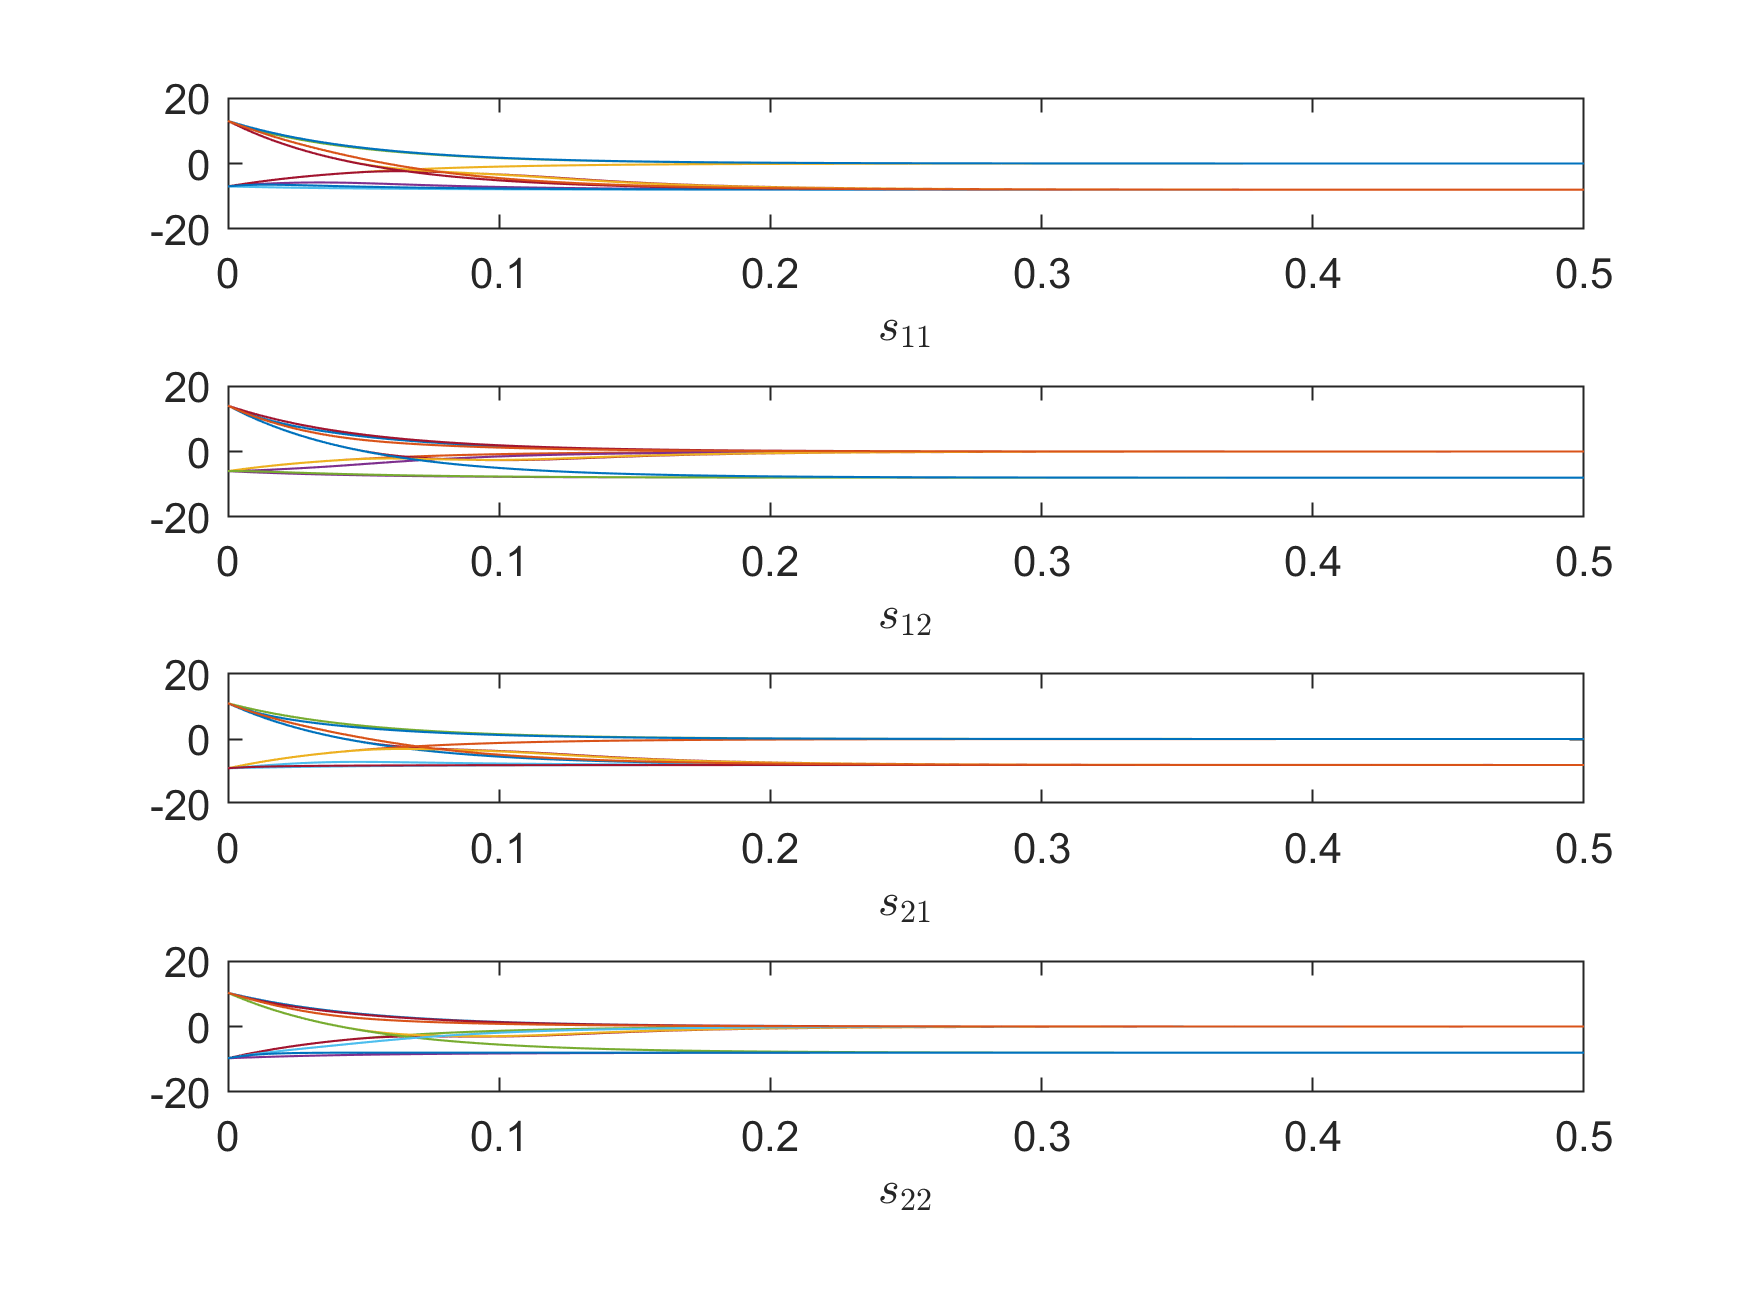
\includegraphics[width=\textwidth]{text/analysis/fig/2by2monotone/s_2.png}
    \caption{Original system \eqref{eq:cl_loop} simulation with several initial conditions}
    \label{fig:s_mono_two}
\end{figure}
        
    
\paragraph{Effect of biases $\beta$} It is interesting to study the effect of the bias parameters $\beta_1,\beta_2 $ on the number of equilibria and the size of the basin of attraction. In particular, we will consider the effect of the biases both for $\alpha<\alpha^* $ and also for $\alpha>\alpha^* $ (system with coupling above bifurcation threshold). 

When $\alpha<\alpha^*$ changing the bias parameters $\beta_1, \beta_2$ does not affect the qualitative behaviour of the system. In fact, the only effect is the one of changing the position of the attractor of the state space.

When $\alpha>\alpha^*$ changing the bias parameters $\beta_1, \beta_2$ moves the equilibria in such a way that a \textbf{saddle-node bifurcation} occurs.
Since the original system in \eqref{eq:cl_loop} is symmetric with respect to the choice of $s_1$ or $s_2$ we can study the effect of changing the bias terms by studying $\beta_2$ and keeping constant $\beta_1$. Furthermore, varying both $\beta_{21}$ and $\beta_{22}$ is not particularly interesting since what determines the behaviour of the system is the difference  $\beta_{21} - \beta_{22}$. Therefore, for simplicity we are gonna study the effect of varying the bias $\beta_{21}$. 

Increasing $\beta_{21}$ (in a neurobiological framework this corresponds to a higher level of self-excitation) the basin of attraction corresponding to the equilibrium $(1, 0)$ expands until a \textbf{saddle-node bifurcation} occurs (refer to section in the preliminaries). This can be intuitively interpreted as follows: by increasing the self-activation of one unit, the basin of attraction corresponding to the pattern in which the corresponding unit is active expands at the expenses of the other attractors until they eventually get completely 'adsorbed'. In \cref{fig:two_d_system_bias_effect} this effect is visible with the help of the phase portrait analysis. (Plot could be improved with a better legend, maybe)

\iftrue
   \begin{figure*}
        %\centering
        \begin{subfigure}[b]{0.475\textwidth}
            \centering
            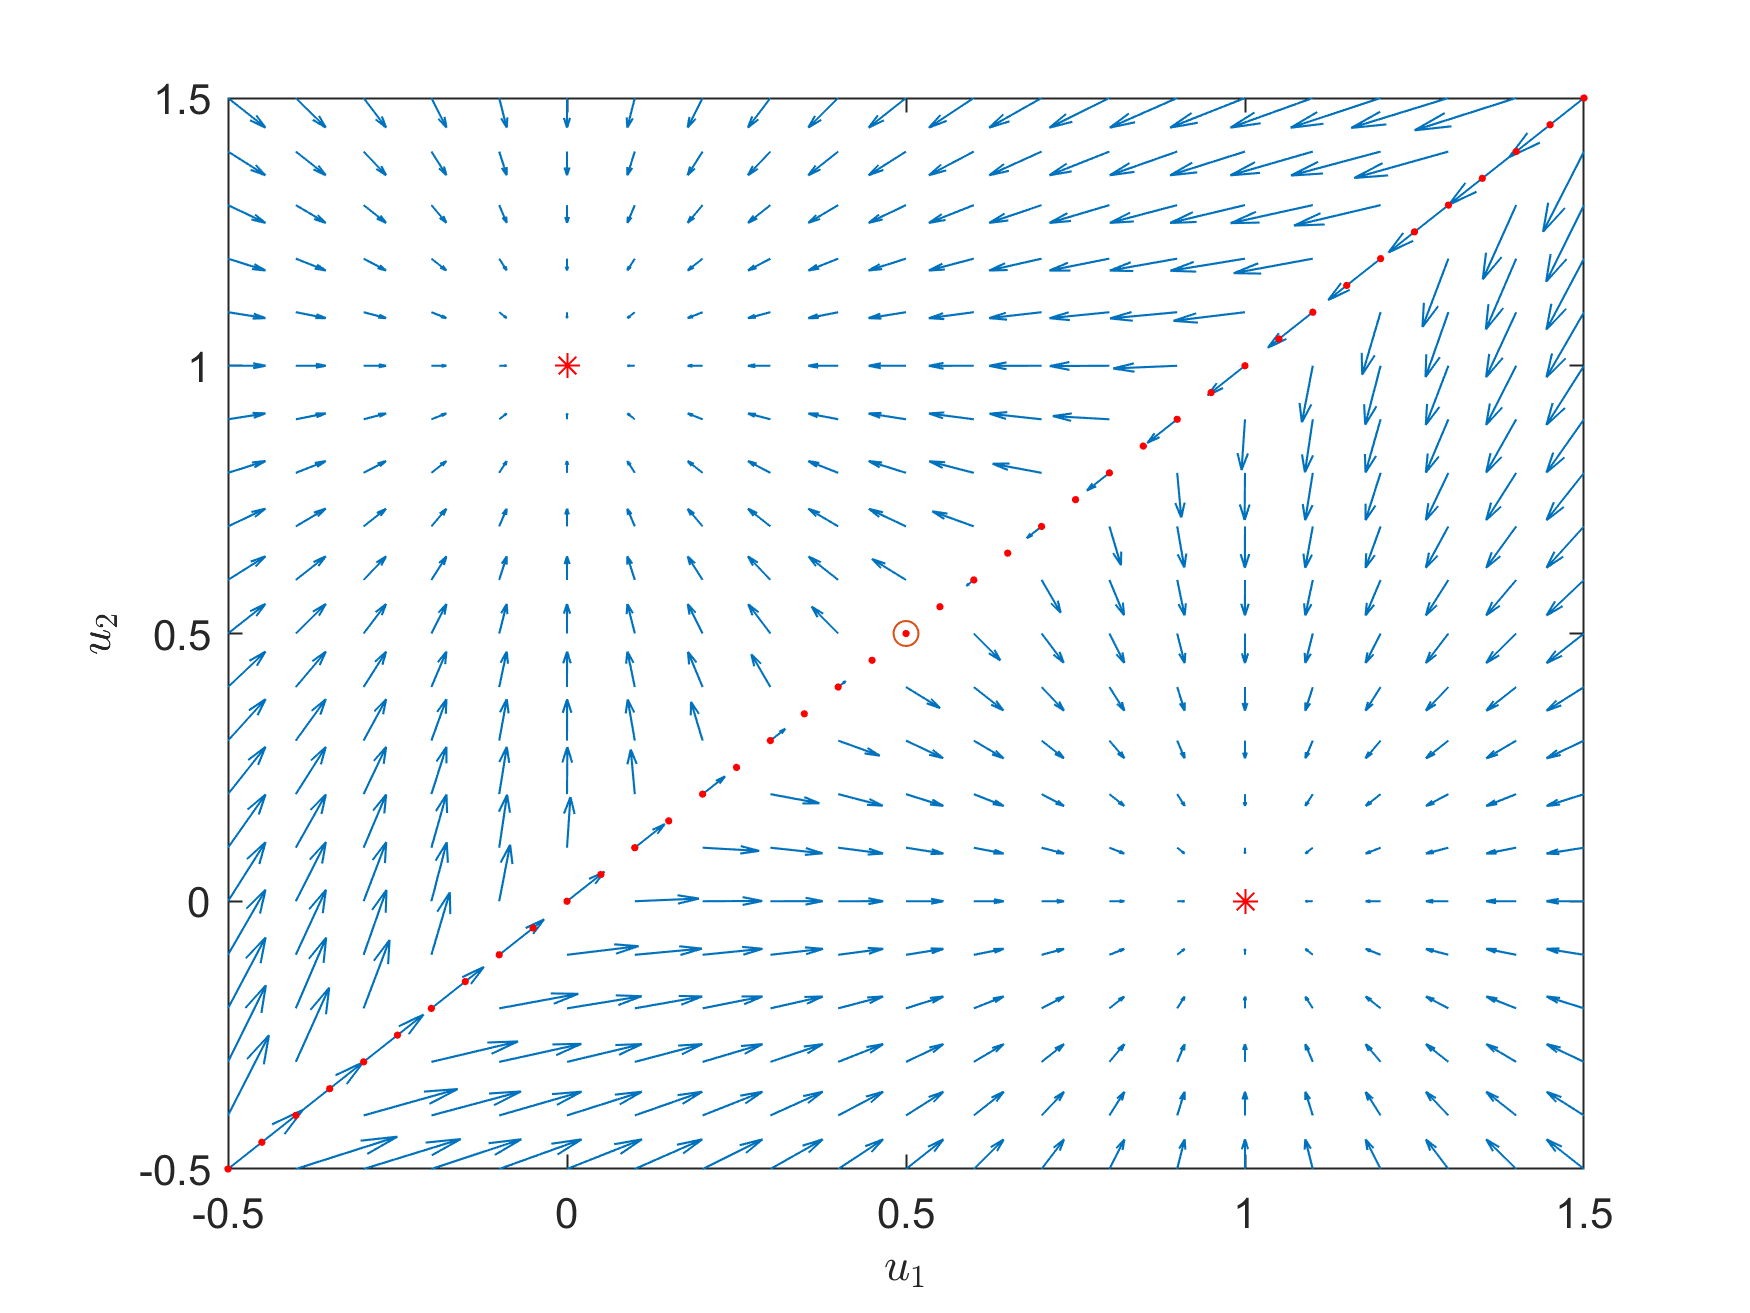
\includegraphics[width=\textwidth]{text/analysis/fig/2by2monotone/bias_0.png}
            \caption{\small $\beta_{21}=0$}
            \label{fig:mean and std of net14}
        \end{subfigure}
        \hfill
        \begin{subfigure}[b]{0.475\textwidth}  
            \centering 
            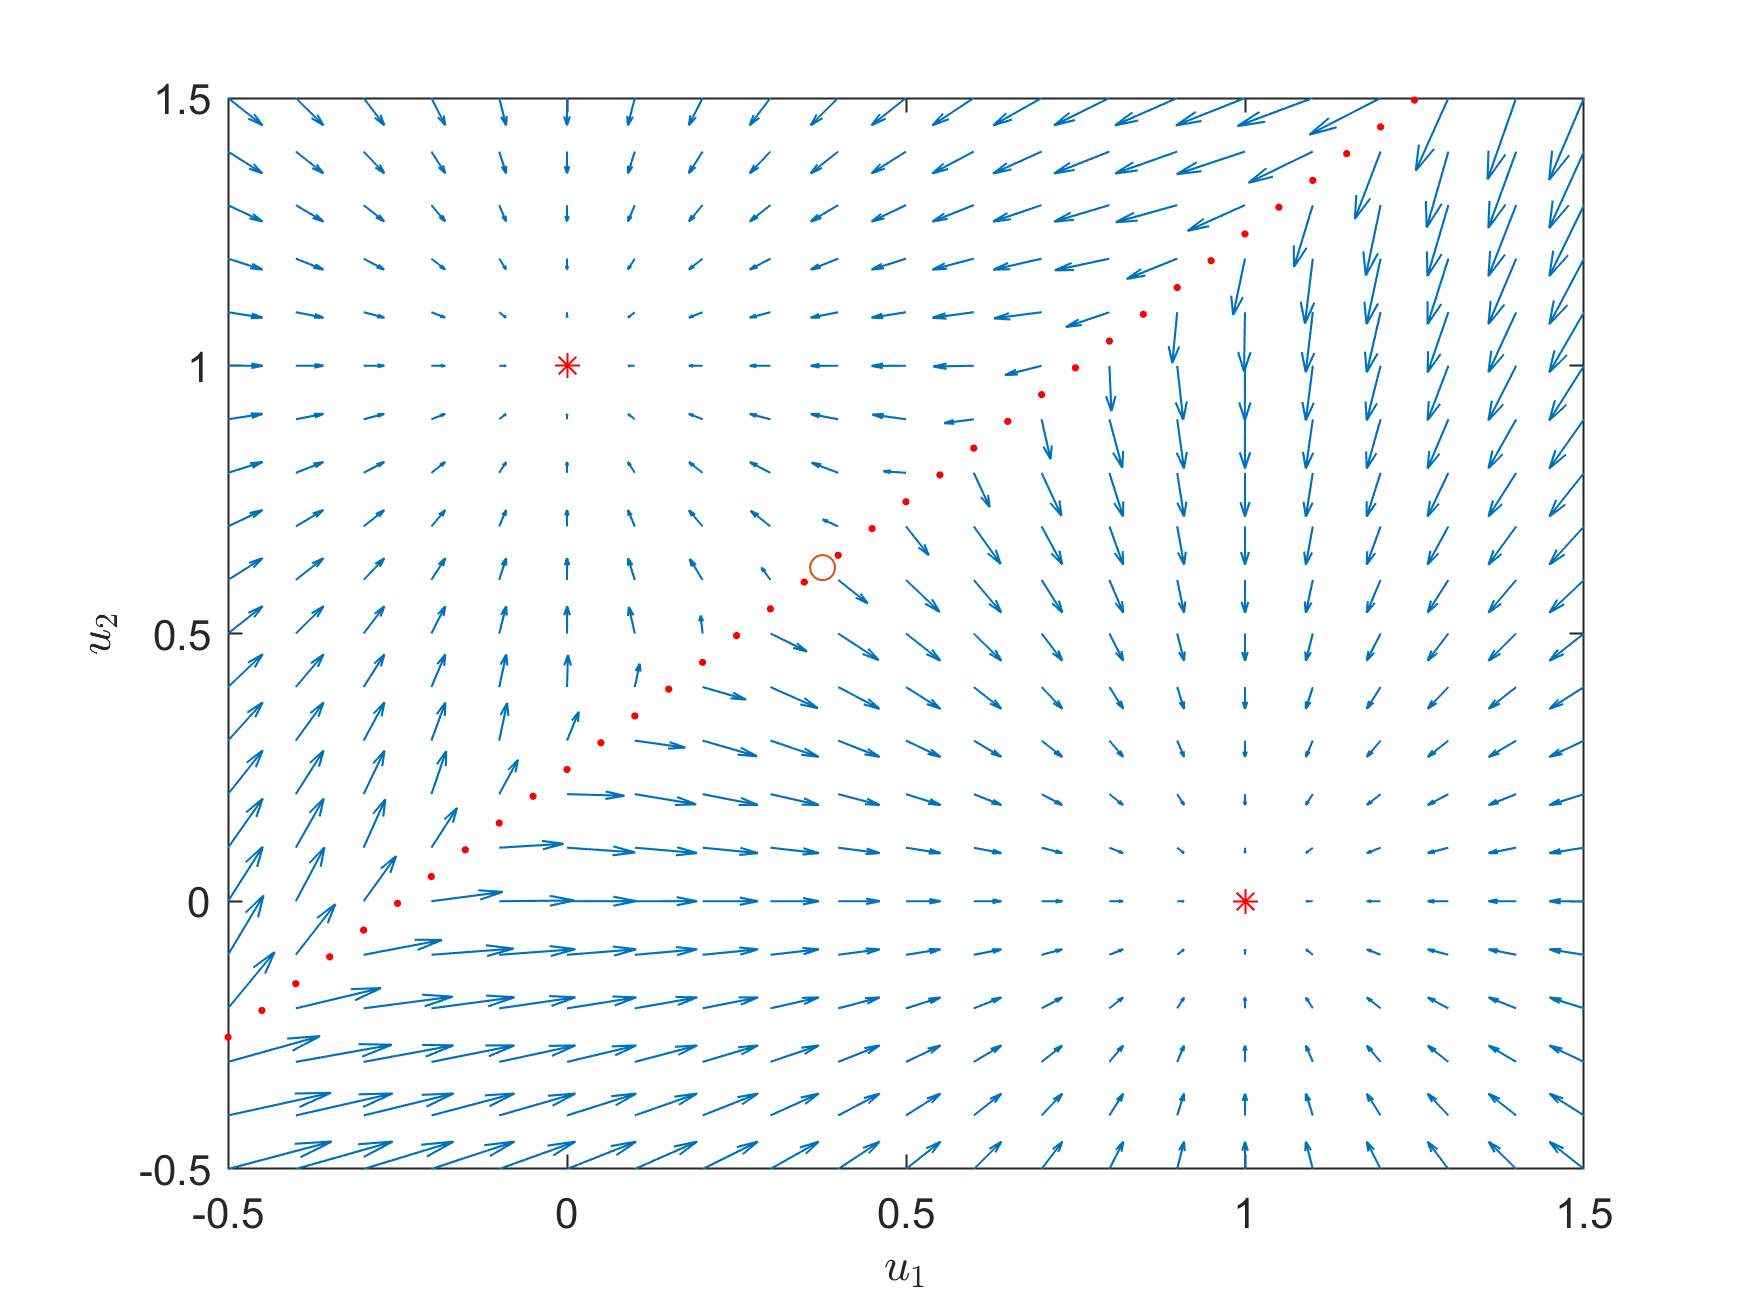
\includegraphics[width=\textwidth]{text/analysis/fig/2by2monotone/bias_2.png}
            \caption{$\beta_{21}=2$}
            \label{fig:mean and std of net24}
        \end{subfigure}
        \vskip\baselineskip
        \begin{subfigure}[b]{0.475\textwidth}   
            \centering 
            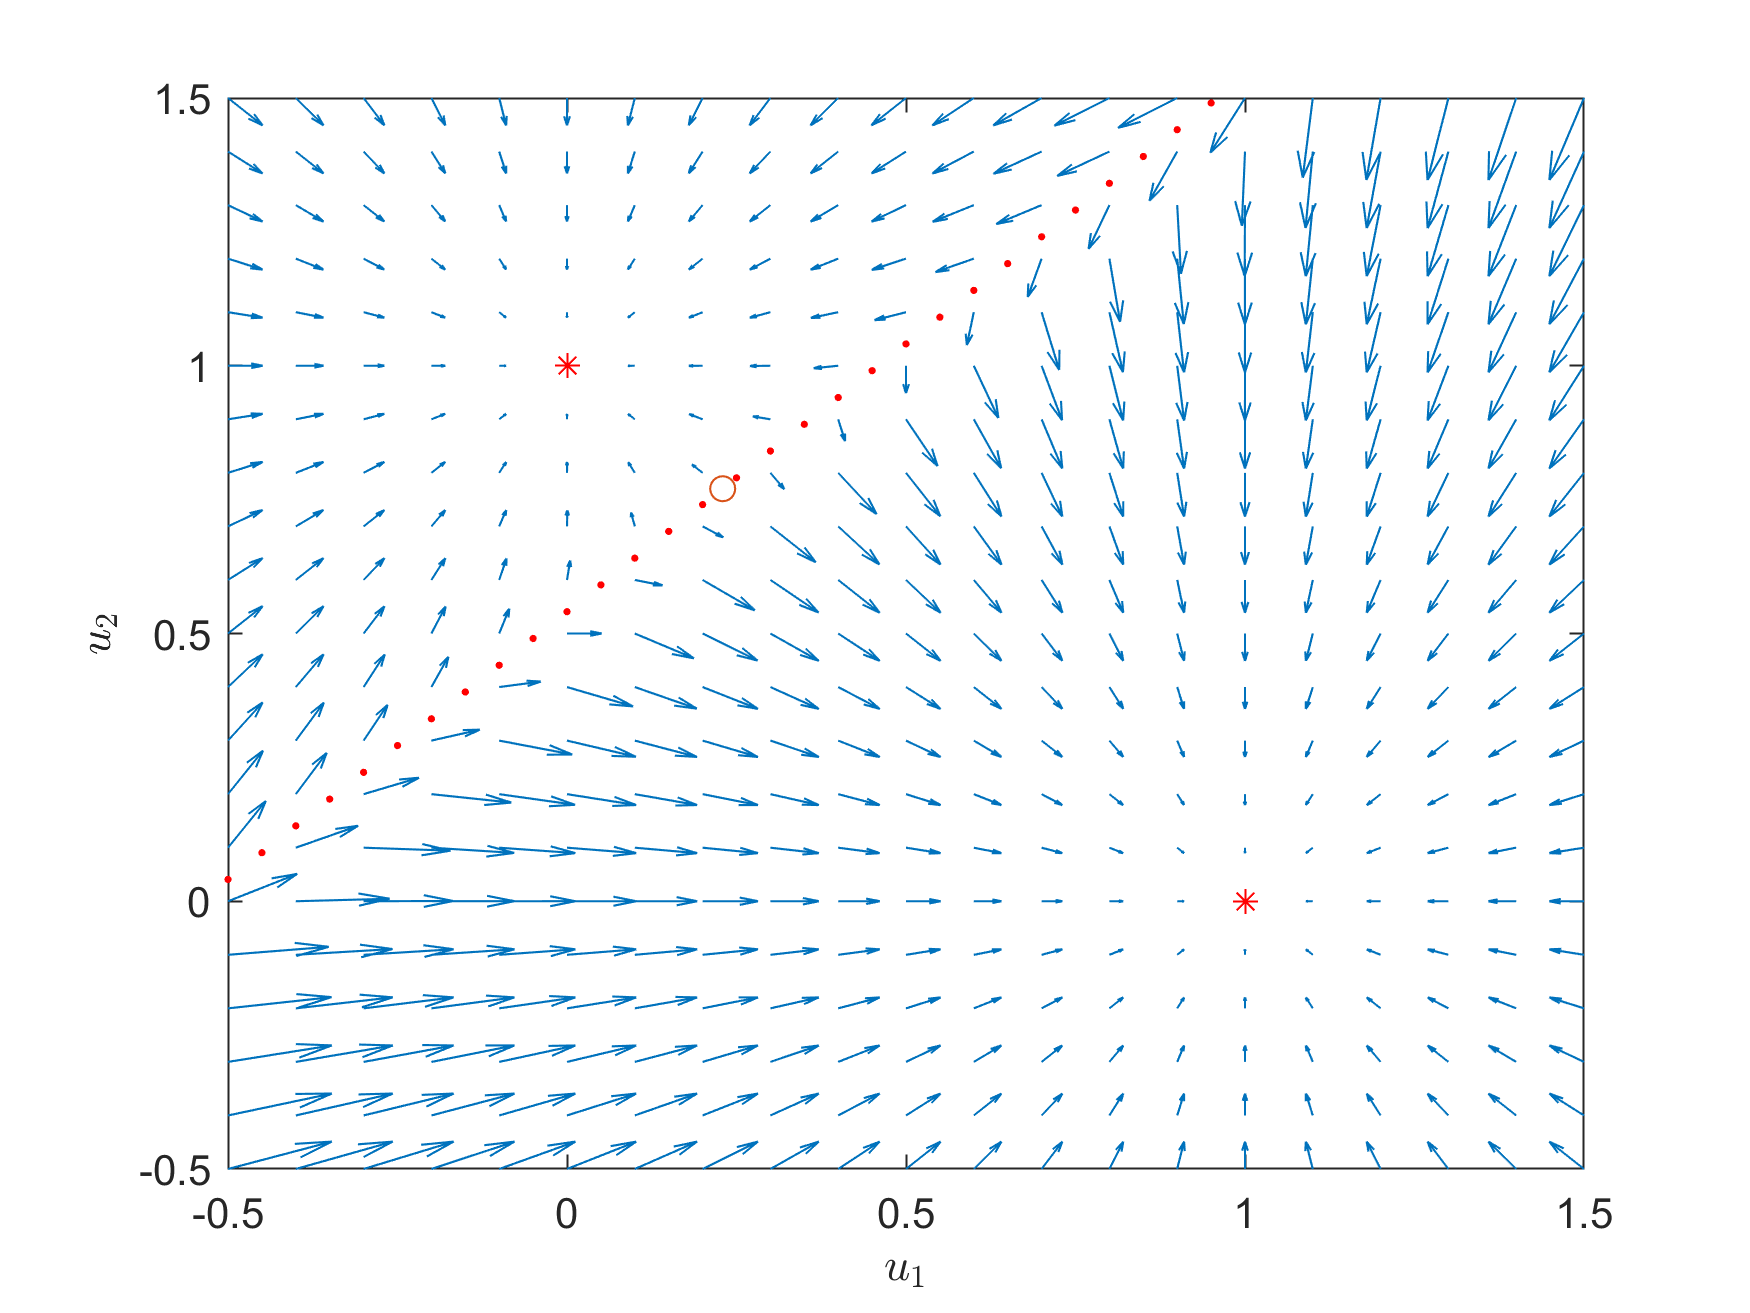
\includegraphics[width=\textwidth]{text/analysis/fig/2by2monotone/bias_4.png}
            \caption{$\beta_{21}=4$}
            \label{fig:mean and std of net34}
        \end{subfigure}
        \quad
        \begin{subfigure}[b]{0.475\textwidth}   
            \centering 
            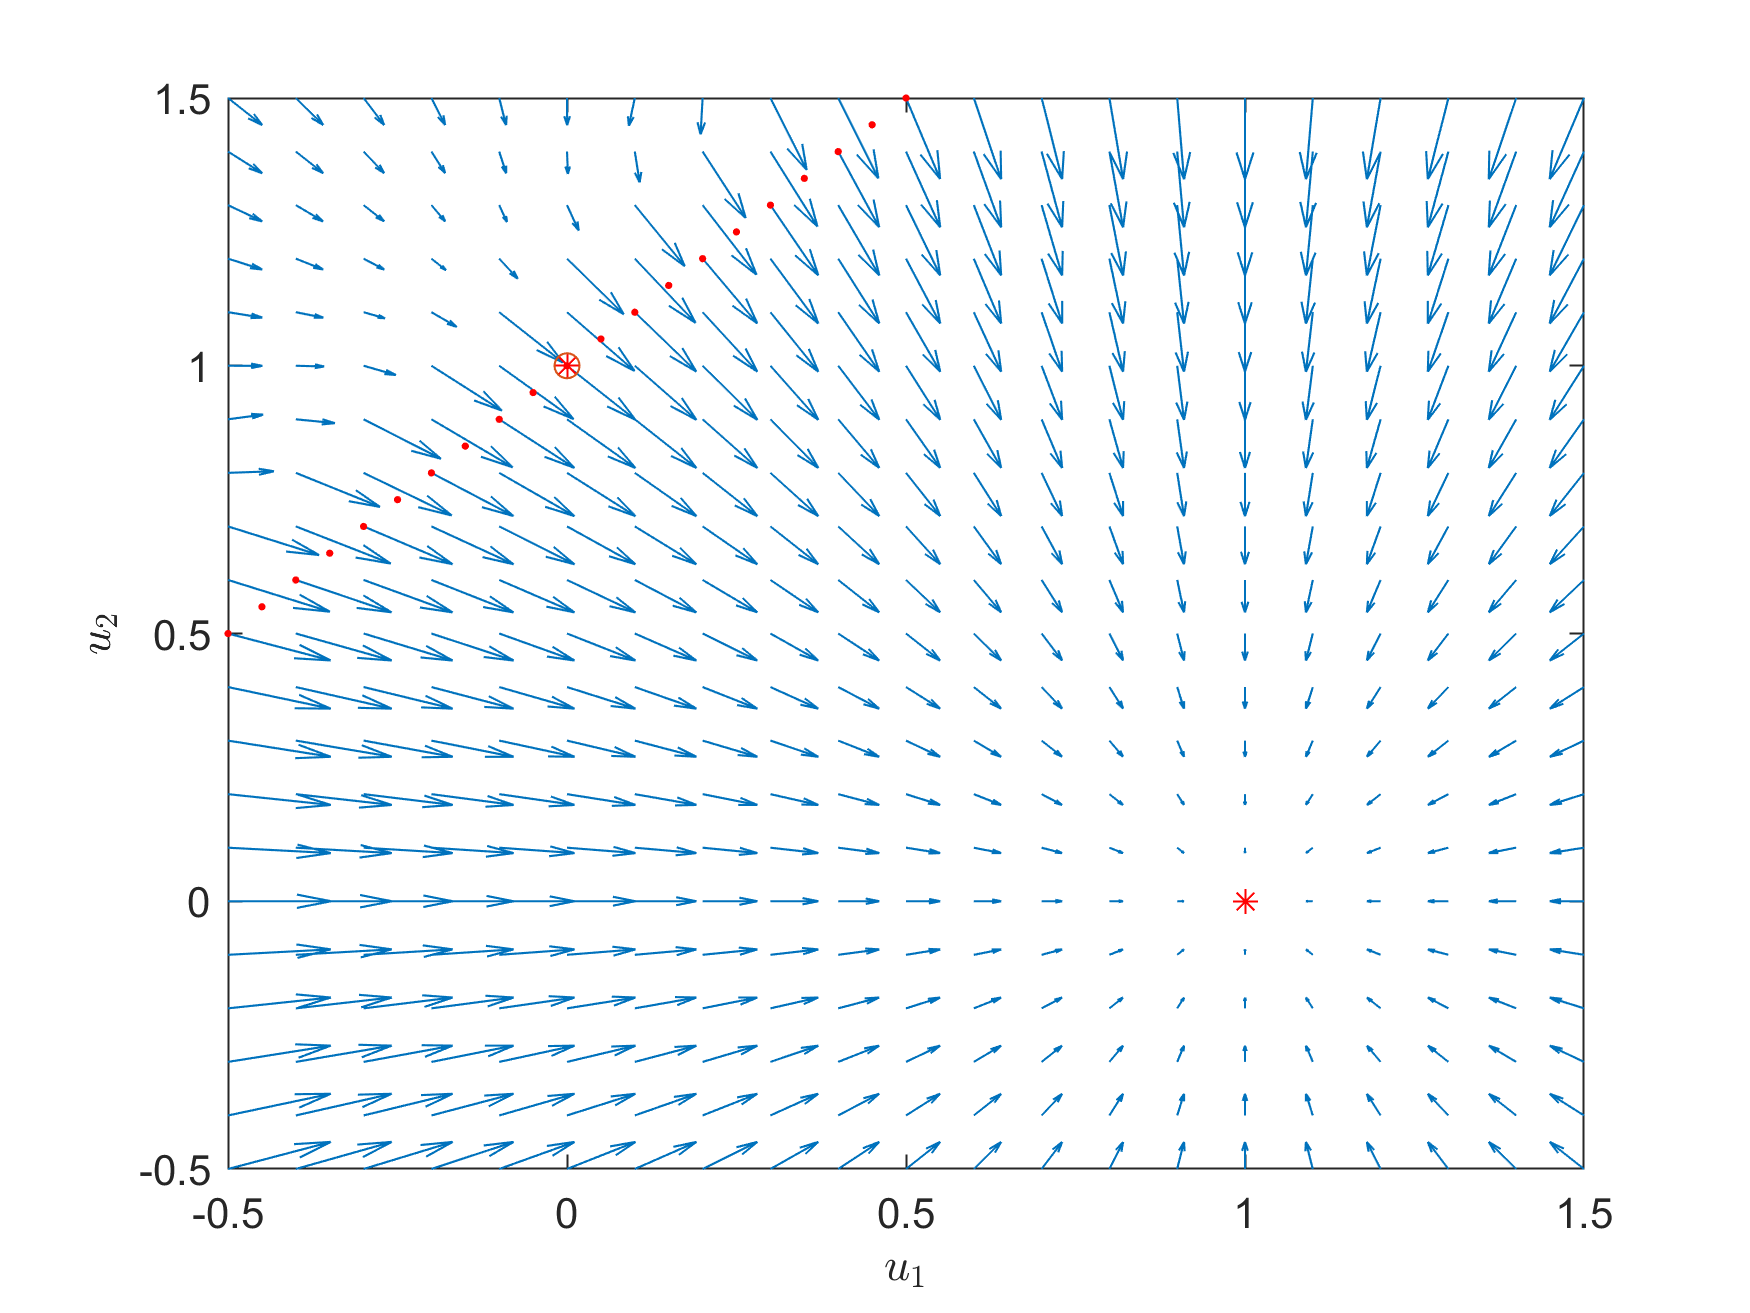
\includegraphics[width=\textwidth]{text/analysis/fig/2by2monotone/bias_10.png}
            \caption{$\beta_{21}=10$}
            \label{fig:mean and std of net44}
        \end{subfigure}
        \caption{Phase portrait for the system in \eqref{eq:reduced_2d} with different coupling factors. $u=[u_1, u_2]^T$} 
        \label{fig:two_d_system_bias_effect}
    \end{figure*}
\fi

\paragraph{Limitations} We have seen so far how the Monotonicity analysis of this section helped us to reduce the complexity of our 4-dimensional system, allowing us to study a 2-dimensional system. Furthermore, we got some interesting insight on the role of the dynamics parameters $\alpha$ and $\beta$. Unfortunately, this approach can not be easily extended to a system with a higher number of dimensions and can not be applied to a system with negative loops as we will see when we will add the adaptation module.